\documentclass[aspectratio=169,11pt,t]{beamer}

% ==============================================================================
% PACKAGES
% ==============================================================================
\usepackage[utf8]{inputenc}
\usepackage[T1]{fontenc}
\usepackage[french]{babel}
\usepackage{lmodern}
\usepackage{amsmath,amssymb}
\usepackage{graphicx}
\usepackage{booktabs}
\usepackage{array}
\usepackage{listings}
\usepackage{tikz}
\usetikzlibrary{arrows.meta,positioning,calc,shapes.geometric}

% ==============================================================================
% CHARTE : bleu marine + gris, un seul accent doré (filets et numéros)
% ==============================================================================
\definecolor{navy}{RGB}{26,54,93}
\definecolor{gold}{RGB}{201,150,46}
\definecolor{ink}{RGB}{38,44,56}
\definecolor{mid}{RGB}{105,112,125}
\definecolor{lightbg}{RGB}{241,243,247}

\usetheme{default}
\setbeamertemplate{navigation symbols}{}
\setbeamercolor{normal text}{fg=ink,bg=white}
\setbeamercolor{structure}{fg=navy}
\setbeamercolor{item}{fg=navy}
\setbeamercolor{itemize item}{fg=navy}
\setbeamercolor{itemize subitem}{fg=mid}
\setbeamercolor{enumerate item}{fg=navy}
\setbeamercolor{block title}{fg=white,bg=navy}
\setbeamercolor{block body}{fg=ink,bg=lightbg}
\setbeamercolor{headline}{fg=white,bg=navy}
\setbeamercolor{caption name}{fg=mid}
\setbeamerfont{caption}{size=\scriptsize}
\setbeamertemplate{itemize item}{\raisebox{0.15ex}{\scalebox{0.7}{$\blacksquare$}}}
\setbeamertemplate{itemize subitem}{\raisebox{0.15ex}{\scalebox{0.6}{$\blacksquare$}}}
\setbeamertemplate{enumerate item}[default]
\setbeamertemplate{blocks}[rounded][shadow=false]
\setbeamerfont{block title}{series=\bfseries,size=\small}

% --- Bandeau de titre (navy) + filet doré ---
\makeatletter
\gdef\currtitle{}
\setbeamertemplate{frametitle}{\protected@xdef\currtitle{\insertframetitle}}
\makeatother
\setbeamertemplate{headline}{%
    \leavevmode%
    \begin{beamercolorbox}[wd=\paperwidth,ht=0.95cm,dp=0.3cm,leftskip=0.8cm,rightskip=0.8cm]{headline}
        {\Large\bfseries\currtitle}\hfill{\footnotesize\color{white!65}\insertsection}
    \end{beamercolorbox}%
    \vskip0pt{\color{gold}\hrule height 1.4pt}%
}

% --- Pied de page discret ---
\setbeamertemplate{footline}{%
    \leavevmode\hbox to\paperwidth{\hspace{0.8cm}%
    {\color{mid}\tiny Groupe 5 \;|\; ENSGMM1 -- UNSTIM \;|\; Outils de calcul scientifique}%
    \hfill
    \colorbox{navy}{\color{white}\footnotesize\bfseries\hspace{2pt}\insertframenumber\hspace{2pt}}\hspace{0.3cm}}%
    \vskip0.25cm
}

% --- Pages de section ---
\AtBeginSection[]{%
    \begin{frame}[plain]
    \begin{tikzpicture}[remember picture,overlay]
        \fill[navy] (current page.south west) rectangle (current page.north east);
        \node[anchor=west,text=gold,font=\fontsize{64}{64}\selectfont\bfseries] at ($(current page.west)+(1.6cm,0.2cm)$) {\thesection};
        \draw[gold,line width=1.4pt] ($(current page.west)+(4.4cm,-1.0cm)$) -- ($(current page.west)+(4.4cm,1.4cm)$);
        \node[anchor=west,text=white,font=\fontsize{28}{32}\selectfont\bfseries,align=left,text width=0.72\paperwidth] at ($(current page.west)+(4.9cm,0.2cm)$) {\insertsection};
    \end{tikzpicture}
    \end{frame}}

% --- Macros ---
\newcommand{\Rzero}{\mathcal{R}_0}
\newcommand{\takeaway}[1]{\vfill\noindent{\color{gold}\vrule width 3pt}\colorbox{lightbg}{\parbox[c]{\dimexpr\textwidth-3pt-2\fboxsep\relax}{\vphantom{Ég}\small\textbf{\color{navy}À retenir\,:} #1\vphantom{Ég}}}\par}
\newcommand{\kpi}[2]{%
    \begin{tikzpicture}\node[draw=navy,line width=0.8pt,rounded corners=3pt,fill=white,minimum width=3.3cm,minimum height=1.45cm,text width=3.0cm,align=center,inner sep=3pt]
    {{\color{navy}\Large\bfseries #1}\\[-1pt]{\scriptsize\color{mid} #2}};\end{tikzpicture}}
\newcommand{\figfull}[2][4.4cm]{\centering\includegraphics[width=0.97\textwidth,height=#1,keepaspectratio]{#2}\par}

\lstset{
    language=Python, basicstyle=\ttfamily\scriptsize, keywordstyle=\bfseries\color{navy},
    commentstyle=\itshape\color{mid}, stringstyle=\color{ink}, backgroundcolor=\color{lightbg},
    frame=none, showstringspaces=false, breaklines=true, xleftmargin=4pt,
}

\begin{document}

% ==============================================================================
% 1. TITRE
% ==============================================================================
\begin{frame}[plain]
    \begin{tikzpicture}[remember picture,overlay]
        \fill[navy] (current page.south west) rectangle (current page.north east);
        % courbe décorative (pic viral puis plateau), discrète
        \begin{scope}[shift={($(current page.south east)+(-6.6cm,0.9cm)$)}]
            \draw[white!22!navy,line width=2.5pt] plot[domain=0:5.8,samples=70,smooth]
                (\x,{0.12*\x+1.3*exp(-((\x-1.6)^2)/0.3)+0.5*exp(-\x/5)});
            \draw[white!15!navy,line width=0.6pt] (0,0)--(5.8,0);
        \end{scope}
        % bandeau blanc institutionnel
        \fill[white] ($(current page.north west)+(0,-2.35cm)$) rectangle (current page.north east);
        \draw[gold,line width=2pt] ($(current page.north west)+(0,-2.35cm)$) -- ($(current page.north east)+(0,-2.35cm)$);
        \node[anchor=west] at ($(current page.north west)+(0.9cm,-1.18cm)$) {
\includegraphics[height=1.55cm]{figures/logo_unstim.png}};
        \node[anchor=east] at ($(current page.north east)+(-0.9cm,-1.18cm)$) {
\includegraphics[height=1.55cm]{figures/logo_ensgmm.png}};
        \node[anchor=center,text=navy,font=\scriptsize,align=center] at ($(current page.north)+(0,-1.18cm)$)
            {\textbf{République du Bénin}\\Université Nationale des Sciences, Technologies,\\Ingénierie et Mathématiques d'Abomey (UNSTIM)\\\textbf{École Nationale Supérieure de Génie Mathématique}\\\textbf{et Modélisation (ENSGMM)}};
        % titre
        \node[anchor=north west,text=gold,font=\footnotesize\bfseries] at ($(current page.north west)+(0.9cm,-2.75cm)$) {UE : OUTILS DE CALCUL SCIENTIFIQUE};
        \node[anchor=north west,text=white,font=\fontsize{23}{27}\selectfont\bfseries,align=left,text width=0.8\paperwidth] at ($(current page.north west)+(0.9cm,-3.25cm)$)
            {Implémentation du modèle d'infection par le VIH-SIDA};
        \draw[gold,line width=1.8pt] ($(current page.north west)+(0.9cm,-5.25cm)$) -- ($(current page.north west)+(4.5cm,-5.25cm)$);
        \node[anchor=north west,text=white!85,font=\itshape\footnotesize,align=left,text width=0.82\paperwidth] at ($(current page.north west)+(0.9cm,-5.4cm)$)
            {Analyse mathématique, stabilité et résolution numérique avec BLAS, LAPACK et Intel MKL};
        % auteurs
        \node[anchor=south west,text=white,font=\scriptsize,align=left] at ($(current page.south west)+(0.9cm,0.45cm)$)
            {\textcolor{gold}{\textbf{Présenté par le Groupe 5}}\\ADOGOUN Déo Gracias Mahugnon\\BIAHOU Ahossou Junior Marie-Clémenceau\\SYLLA IMOROU Izou Dine};
        \node[anchor=south east,text=white!85,font=\scriptsize,align=right] at ($(current page.south east)+(-0.9cm,0.45cm)$)
            {\textcolor{gold}{\textbf{Sous la direction du}}\\Dr. Carlos AGOSSOU\\Promotion ENSGMM1};
    \end{tikzpicture}
\end{frame}

% ==============================================================================
% 2. PLAN
% ==============================================================================
\begin{frame}{Plan de la présentation}
    \vspace{0.2cm}
    \begin{tikzpicture}
        \draw[gold,line width=1pt] (-0.5,0.55) -- (-0.5,-5.0);
        \node[circle,fill=navy,text=white,font=\bfseries,minimum size=0.75cm,inner sep=0pt] at (0,0.00) {1};
        \node[anchor=west,font=\large\bfseries,text=navy] at (0.65,0.12) {Outils : MKL, BLAS, LAPACK};
        \node[anchor=west,font=\footnotesize,text=mid] at (0.65,-0.22) {La pile logicielle de calcul scientifique};
        \node[circle,fill=navy,text=white,font=\bfseries,minimum size=0.75cm,inner sep=0pt] at (0,-0.98) {2};
        \node[anchor=west,font=\large\bfseries,text=navy] at (0.65,-0.86) {Modèle intra-hôte};
        \node[anchor=west,font=\footnotesize,text=mid] at (0.65,-1.20) {Équations, $\Rzero$, stabilité chez un patient};
        \node[circle,fill=navy,text=white,font=\bfseries,minimum size=0.75cm,inner sep=0pt] at (0,-1.96) {3};
        \node[anchor=west,font=\large\bfseries,text=navy] at (0.65,-1.84) {Calcul numérique};
        \node[anchor=west,font=\footnotesize,text=mid] at (0.65,-2.18) {Conditionnement, Newton, raideur, Euler implicite};
        \node[circle,fill=navy,text=white,font=\bfseries,minimum size=0.75cm,inner sep=0pt] at (0,-2.94) {4};
        \node[anchor=west,font=\large\bfseries,text=navy] at (0.65,-2.82) {Résultats médicaux};
        \node[anchor=west,font=\footnotesize,text=mid] at (0.65,-3.16) {Primo-infection, traitement, rebond};
        \node[circle,fill=navy,text=white,font=\bfseries,minimum size=0.75cm,inner sep=0pt] at (0,-3.92) {5};
        \node[anchor=west,font=\large\bfseries,text=navy] at (0.65,-3.80) {Modèle de population};
        \node[anchor=west,font=\footnotesize,text=mid] at (0.65,-4.14) {Propagation de l'épidémie, prévention et traitement};
        \node[circle,fill=navy,text=white,font=\bfseries,minimum size=0.75cm,inner sep=0pt] at (0,-4.90) {6};
        \node[anchor=west,font=\large\bfseries,text=navy] at (0.65,-4.78) {Performance};
        \node[anchor=west,font=\footnotesize,text=mid] at (0.65,-5.12) {Gain de vitesse de BLAS/LAPACK};
    \end{tikzpicture}
\end{frame}

% ==============================================================================
\section{Outils : MKL, BLAS, LAPACK}

\begin{frame}{Problématique et objectifs}
    \begin{columns}[T,onlytextwidth]
        \begin{column}{0.46\textwidth}
            \begin{block}{Question}
                Comment le VIH se propage-t-il chez un patient et dans une population, et à partir de quelle efficacité un traitement l'arrête-t-il ?
            \end{block}
            \vspace{0.2cm}
            \textbf{Deux échelles de modélisation}
            \medskip

            \begin{tikzpicture}
                \node[draw=navy,rounded corners=3pt,minimum width=3.0cm,minimum height=1.1cm,align=center,font=\small] {\textbf{Patient}\\jours : $T, I, V$};
                \node[draw=navy,rounded corners=3pt,minimum width=3.0cm,minimum height=1.1cm,align=center,font=\small] at (3.4,0) {\textbf{Population}\\années : $S, I_1, I_2$};
            \end{tikzpicture}
        \end{column}
        \begin{column}{0.5\textwidth}
            \textbf{Quatre objectifs}
            \medskip
            \begin{enumerate}
                \item Maîtriser la pile \textbf{MKL / BLAS / LAPACK} depuis Python.
                \item Analyser les modèles : $\Rzero$ et stabilité.
                \item Les résoudre avec \texttt{DGESV}, \texttt{DGEEQU}, \texttt{DGEEV} et interpréter médicalement.
                \item Mesurer le gain de performance.
            \end{enumerate}
            \vspace{0.2cm}
            Des équations \textbf{non linéaires et raides} : impossibles à résoudre à la main.
        \end{column}
    \end{columns}
    \takeaway{un problème médical qui exige des solveurs fiables et rapides.}
\end{frame}

\begin{frame}{La pile logicielle : qui fait quoi ?}
    \begin{columns}[T,onlytextwidth]
        \begin{column}{0.46\textwidth}
            \centering\vspace{-0.1cm}
            \begin{tikzpicture}[
                box/.style={rectangle,draw=navy,fill=lightbg,minimum width=4.8cm,minimum height=0.55cm,align=center,font=\footnotesize},
                top/.style={box,fill=navy,text=white},
                arr/.style={-{Stealth[length=2mm]},color=navy,thick}]
                \node[top] (a) {Modèles du VIH (équations différentielles)};
                \node[box,below=0.2cm of a] (b) {Python : NumPy / SciPy};
                \node[box,below=0.2cm of b] (c) {LAPACK : \texttt{DGESV}, \texttt{DGEEV}, \dots};
                \node[box,below=0.2cm of c] (d) {BLAS : \texttt{DGEMM}, \texttt{DAXPY}, \dots};
                \node[box,below=0.2cm of d,draw=gold,line width=1pt] (e) {Intel MKL ou OpenBLAS (processeur)};
                \draw[arr] (a)--(b); \draw[arr] (b)--(c); \draw[arr] (c)--(d); \draw[arr] (d)--(e);
            \end{tikzpicture}
        \end{column}
        \begin{column}{0.5\textwidth}\small
            \begin{itemize}
                \item \textbf{BLAS} : spécification des opérations de base.
                \item \textbf{LAPACK} : résout $Ax=b$, valeurs propres, etc., via BLAS.
                \item \textbf{Intel MKL} : implémentation optimisée des deux.
                \item Alternatives : OpenBLAS, BLIS, Netlib.
            \end{itemize}
        \end{column}
    \end{columns}
    \takeaway{le code appelant reste le même ; seule l'implémentation change.}
\end{frame}

\begin{frame}{BLAS : trois niveaux, une idée clé}
    \begin{columns}[T,onlytextwidth]
        \begin{column}{0.62\textwidth}
            \small
            \begin{tabular}{c l c c l}
                \toprule
                \textbf{Niv.} & \textbf{Opération} & \textbf{Données} & \textbf{Calculs} & \textbf{Routine}\\
                \midrule
                1 & vecteur--vecteur & $O(n)$ & $O(n)$ & \texttt{DAXPY}\\
                2 & matrice--vecteur & $O(n^2)$ & $O(n^2)$ & \texttt{DGEMV}\\
                3 & matrice--matrice & $O(n^2)$ & $O(n^3)$ & \texttt{DGEMM}\\
                \bottomrule
            \end{tabular}
            \medskip
            \begin{itemize}
                \item Nom d'une routine : \texttt{[Précision][Type][Opération]}.
                \item \texttt{DGEMM} = \textbf{D}ouble, \textbf{GE}nérale, \textbf{M}atrice-\textbf{M}atrice.
            \end{itemize}
        \end{column}
        \begin{column}{0.34\textwidth}
            \centering
            \kpi{$O(n)$}{opérations par donnée au niveau 3}
        \end{column}
    \end{columns}
    \takeaway{au niveau 3, les blocs de données sont réutilisés dans le cache : le processeur travaille à pleine vitesse.}
\end{frame}

\begin{frame}{LAPACK : les routines du projet}
    \centering\small
    \begin{tabular}{l l l}
        \toprule
        \textbf{Problème} & \textbf{Routine} & \textbf{Méthode}\\
        \midrule
        Résoudre $Ax=b$ & \texttt{DGESV} & factorisation LU, pivotage partiel\\
        Équilibrer une matrice & \texttt{DGEEQU} & mise à l'échelle lignes/colonnes\\
        Estimer le conditionnement & \texttt{DGECON} & estimation de $\|A^{-1}\|_1$\\
        Valeurs propres & \texttt{DGEEV} & Hessenberg + algorithme QR\\
        Valeurs singulières & \texttt{DGESDD} & diviser pour régner\\
        \bottomrule
    \end{tabular}
    \vspace{0.3cm}
    \begin{itemize}
        \item Algorithmes \textbf{par blocs} : le gros du travail est confié à \texttt{DGEMM}.
        \item Précision : l'erreur peut atteindre $\kappa(A)\,\varepsilon_{\mathrm{mach}}$ avec $\varepsilon_{\mathrm{mach}}\approx10^{-16}$.
    \end{itemize}
    \takeaway{LAPACK fournit, en un appel, factorisation, spectre et conditionnement.}
\end{frame}

\begin{frame}[fragile]{Utilisation depuis Python}
    \begin{columns}[T,onlytextwidth]
        \begin{column}{0.58\textwidth}
            \begin{lstlisting}
import numpy as np
from scipy.linalg import lapack
from threadpoolctl import threadpool_info

print(threadpool_info())   # openblas ou mkl ?

A = np.asfortranarray([[3., 1.], [1., 2.]])
b = np.array([9., 8.])

lu, piv, x, info = lapack.dgesv(A, b)   # Ax = b
assert info == 0                        # 0 = succes
wr, wi, vl, vr, info = lapack.dgeev(A)  # valeurs propres
            \end{lstlisting}
        \end{column}
        \begin{column}{0.38\textwidth}
            \begin{itemize}
                \item \texttt{threadpoolctl} identifie le backend actif.
                \item Stockage \textbf{Fortran} (par colonnes) : aucune copie.
                \item \texttt{info} : code d'erreur à toujours tester.
            \end{itemize}
        \end{column}
    \end{columns}
    \takeaway{les routines Fortran d'origine sont appelées directement depuis Python.}
\end{frame}

% ==============================================================================
\section{Modèle intra-hôte}

\begin{frame}{Le VIH : trois phases chez un patient non traité}
    \vspace{0.3cm}
    \centering
    \begin{tikzpicture}[
        ph/.style={rectangle,draw=navy,fill=lightbg,rounded corners=3pt,minimum width=3.7cm,minimum height=2.2cm,align=center,text width=3.4cm,font=\footnotesize},
        arr/.style={-{Stealth[length=2.5mm]},color=gold,line width=1.4pt}]
        \node[ph] (a) {\textbf{\normalsize Phase aiguë}\\[2pt]multiplication explosive,\\pic de charge virale,\\chute des CD4+};
        \node[ph,right=0.8cm of a] (b) {\textbf{\normalsize Phase chronique}\\[2pt]niveau quasi stationnaire,\\sans symptôme,\\destruction lente};
        \node[ph,right=0.8cm of b] (c) {\textbf{\normalsize Stade SIDA}\\[2pt]CD4+ sous $\approx200/\mu$L,\\maladies\\opportunistes};
        \draw[arr] (a)--(b); \draw[arr] (b)--(c);
    \end{tikzpicture}

    \vspace{0.4cm}
    \begin{itemize}
        \item Le virus infecte les \textbf{lymphocytes T CD4+}, qui coordonnent l'immunité, les détourne pour se multiplier, puis ils meurent.
    \end{itemize}
    \takeaway{la phase aiguë est celle que le modèle intra-hôte doit reproduire et que le traitement cherche à stopper.}
\end{frame}

\begin{frame}{Le modèle intra-hôte $(T,I,V)$}
    \begin{columns}[T,onlytextwidth]
        \begin{column}{0.5\textwidth}
            \vspace{0.1cm}
            \[
            \begin{cases}
            \dot T = s - dT - (1-\eta)\beta TV\\[3pt]
            \dot I = (1-\eta)\beta TV - \delta I\\[3pt]
            \dot V = pI - cV
            \end{cases}
            \]
            \footnotesize
            $T$ CD4+ sains \;|\; $I$ cellules infectées \;|\; $V$ virions libres\\
            $\eta\in[0,1]$ : efficacité du traitement
        \end{column}
        \begin{column}{0.48\textwidth}
            \centering
            \begin{tikzpicture}[
                c/.style={rectangle,draw=navy,fill=lightbg,minimum width=1.45cm,minimum height=0.85cm,align=center,font=\footnotesize\bfseries},
                r/.style={-{Stealth[length=2mm]},color=navy,thick}]
                \node[c] (T) {$T$}; \node[c,right=1.1cm of T] (I) {$I$}; \node[c,right=1.1cm of I] (V) {$V$};
                \node[left=0.5cm of T] (s) {}; \node[below=0.7cm of T] (dT) {}; \node[below=0.7cm of I] (dI) {}; \node[below=0.7cm of V] (dV) {};
                \draw[r] (s)--node[above,font=\scriptsize]{$s$}(T);
                \draw[r] (T)--node[above,font=\tiny]{$(1-\eta)\beta TV$}(I);
                \draw[r] (I)--node[above,font=\scriptsize]{$pI$}(V);
                \draw[r] (T)--node[left,font=\scriptsize]{$dT$}(dT);
                \draw[r] (I)--node[left,font=\scriptsize]{$\delta I$}(dI);
                \draw[r] (V)--node[left,font=\scriptsize]{$cV$}(dV);
            \end{tikzpicture}
        \end{column}
    \end{columns}
    \vspace{0.2cm}
    \centering\footnotesize
    \begin{tabular}{c c c c c c}
        \toprule
        $s=10$ & $d=0{,}01$ & $\beta=4{,}6\times10^{-5}$ & $\delta=0{,}5$ & $p=1000$ & $c=23$\\
        \bottomrule
    \end{tabular}
    \takeaway{ce système décrit la vie du virus dans un patient ; reste à vérifier qu'il est réaliste.}
\end{frame}

\begin{frame}{Le modèle est-il réaliste ?}
    \begin{columns}[T,onlytextwidth]
        \begin{column}{0.48\textwidth}
            \begin{tikzpicture}
                \node[draw=navy,rounded corners=3pt,fill=lightbg,text width=5.3cm,inner sep=7pt,font=\small] {
                    \textbf{1. Positivité}\\[3pt]
                    Un nombre de cellules ou de virus ne peut \textbf{jamais être négatif}.\\[3pt]
                    \emph{Ici :} quand une population tombe à $0$, ses équations ne la rendent pas négative ; elle repart de $0$ vers le haut.};
            \end{tikzpicture}
        \end{column}
        \begin{column}{0.48\textwidth}
            \begin{tikzpicture}
                \node[draw=navy,rounded corners=3pt,fill=lightbg,text width=5.3cm,inner sep=7pt,font=\small] {
                    \textbf{2. Bornitude}\\[3pt]
                    Les populations ne \textbf{grandissent pas sans limite} : elles restent sous un plafond.\\[3pt]
                    \emph{Ici :} les CD4+ (sains + infectés) ne dépassent jamais $s/d=1000$ cellules par $\mu$L, le niveau d'un sujet sain.};
            \end{tikzpicture}
        \end{column}
    \end{columns}
    \takeaway{le modèle ne produit pas de résultats absurdes : il est biologiquement cohérent.}
\end{frame}

\begin{frame}{Calcul de $\Rzero$ : la matrice de prochaine génération}
    \small
    $\Rzero$ = nombre de \textbf{nouvelles cellules infectées} produites par \textbf{une} cellule infectée dans un organisme sain.
    \vspace{0.2cm}

    \centering
    \begin{tikzpicture}[
        st/.style={rectangle,draw=navy,fill=lightbg,rounded corners=3pt,minimum width=3.3cm,minimum height=1.35cm,align=center,text width=3.1cm,font=\scriptsize},
        arr/.style={-{Stealth[length=2mm]},color=gold,line width=1.2pt}]
        \node[st] (a) {\textbf{1. Séparer}\\ $\mathcal F$ : nouvelles infections\\$\mathcal V$ : le reste (morts, transferts)};
        \node[st,right=0.5cm of a] (b) {\textbf{2. Dériver}\\ $F$, $V_m$ : dérivées partielles premières en $E_0$};
        \node[st,right=0.5cm of b] (c) {\textbf{3. Multiplier}\\ $K=F\,V_m^{-1}$\\(nouvelles infections par infecté)};
        \node[st,right=0.5cm of c] (d) {\textbf{4. Lire}\\ $\Rzero=$ plus grande valeur propre de $K$};
        \draw[arr] (a)--(b); \draw[arr] (b)--(c); \draw[arr] (c)--(d);
    \end{tikzpicture}

    \vspace{0.25cm}
    \begin{columns}[T,onlytextwidth]
        \begin{column}{0.5\textwidth}
            \[
            \mathcal F=\begin{pmatrix}(1-\eta)\beta TV\\0\end{pmatrix}\!,\quad
            \mathcal V=\begin{pmatrix}\delta I\\-pI+cV\end{pmatrix}
            \]
        \end{column}
        \begin{column}{0.5\textwidth}
            \[
            F=\begin{pmatrix}0&(1-\eta)\beta T_0\\0&0\end{pmatrix}\!,\quad
            V_m=\begin{pmatrix}\delta&0\\-p&c\end{pmatrix}
            \]
        \end{column}
    \end{columns}
    \takeaway{on dérive $\mathcal F$ par rapport aux deux variables infectées $(I,V)$ : d'où une matrice $2\times2$.}
\end{frame}

\begin{frame}{Résultat : $\Rzero=4$ et seuil d'efficacité de 75\,\%}
    \vspace{0.1cm}
    \[
    K=\begin{pmatrix}\dfrac{(1-\eta)\beta pT_0}{\delta c}&\dfrac{(1-\eta)\beta T_0}{c}\\[6pt]0&0\end{pmatrix}
    \;\Longrightarrow\;
    \Rzero(\eta)=\frac{(1-\eta)\,\beta\,p\,s}{d\,\delta\,c}
    =\underbrace{\frac p\delta}_{2000\ \text{virions}}\times\underbrace{\frac{(1-\eta)\beta T_0}{c}}_{0{,}002\ \text{cellule}}
    \]
    \vspace{0.1cm}
    \begin{columns}[T,onlytextwidth]
        \begin{column}{0.3\textwidth}\centering\kpi{$\Rzero(0)=4$}{sans traitement}\end{column}
        \begin{column}{0.3\textwidth}\centering\kpi{$\eta_c=75\,\%$}{$1-1/\Rzero(0)$}\end{column}
        \begin{column}{0.36\textwidth}\small
            À $\eta=70\,\%$ : $\Rzero=1{,}2>1$ \\$\Rightarrow$ l'infection persiste.
        \end{column}
    \end{columns}
    \takeaway{un traitement doit bloquer \textbf{au moins 75\,\%} des nouvelles infections pour éliminer le virus.}
\end{frame}

\begin{frame}{Équilibres et stabilité}
    \begin{columns}[T,onlytextwidth]
        \begin{column}{0.46\textwidth}
            \textbf{Deux équilibres}
            \medskip
            \begin{itemize}
                \item \textbf{Sans infection} $E_0=(1000,0,0)$ : stable si $\Rzero<1$.
                \item \textbf{Endémique} $E^*$, si $\Rzero>1$ :
            \end{itemize}
            \[T^*=\tfrac{T_0}{\Rzero}=250,\; I^*=15,\; V^*\approx652\]
            \footnotesize À $\Rzero=1$ : bifurcation transcritique (échange de stabilité).
        \end{column}
        \begin{column}{0.5\textwidth}
            \textbf{Valeurs propres en $E^*$} (\texttt{DGEEV})
            \medskip

            \small
            \begin{tabular}{l l}
                \toprule
                \textbf{Valeur propre} & \textbf{Signification}\\
                \midrule
                $-23{,}50$ & virus libre éliminé en $\approx1$ h\\
                $-0{,}0197\pm0{,}1196\,i$ & oscillations amorties\\
                \bottomrule
            \end{tabular}
            \medskip

            \centering\kpi{$\approx53$ jours}{période des oscillations}
        \end{column}
    \end{columns}
    \takeaway{toutes les parties réelles sont négatives : l'infection chronique est un état stable, approché en oscillant.}
\end{frame}

% ==============================================================================
\section{Calcul numérique}

\begin{frame}{Conditionnement et équilibrage avec \texttt{DGEEQU}}
    \begin{columns}[T,onlytextwidth]
        \begin{column}{0.56\textwidth}
            \begin{itemize}
                \item \texttt{DGESV} donne un résidu $\approx10^{-16}$, mais l'erreur est limitée par $\kappa\,\varepsilon_{\mathrm{mach}}$.
                \item Jacobienne : échelles très différentes ($T\sim10^3$, $p=1000$, $c=23$).
                \item \texttt{DGEEQU} calcule $R$ et $C$ tels que $\widehat J=RJC$.
            \end{itemize}
            \medskip
            \small
            \begin{tabular}{l c c}
                \toprule
                \textbf{Point} & $\kappa_1(J)$ & $\kappa_1(RJC)$\\
                \midrule
                Équilibre endémique $E^*$ & $1{,}5\times10^{5}$ & $\approx69$\\
                Équilibre sain $E_0$ & $1{,}6\times10^{5}$ & $\approx61$\\
                Pic de virémie & $8{,}9\times10^{4}$ & $\approx8$\\
                \bottomrule
            \end{tabular}
        \end{column}
        \begin{column}{0.38\textwidth}
            \centering\vspace{0.4cm}
            \kpi{$10^{5}\;\to\;69$}{$\kappa_1$ à l'équilibre endémique}
        \end{column}
    \end{columns}
    \takeaway{l'équilibrage gagne trois à quatre ordres de grandeur avant toute résolution.}
\end{frame}

\begin{frame}{Méthode de Newton avec \texttt{DGESV}}
    \begin{columns}[T,onlytextwidth]
        \begin{column}{0.44\textwidth}
            Pour trouver un équilibre $f(y^*)=0$ :
            \[J(y_k)\,\delta_k=-f(y_k),\quad y_{k+1}=y_k+\delta_k\]
            \begin{itemize}
                \item Système $3\times3$ résolu par \texttt{DGESV} à chaque itération.
                \item Moins de dix itérations depuis chaque point de départ testé.
                \item Retrouve $E^*=(250;\,15;\,652{,}17)$.
            \end{itemize}
        \end{column}
        \begin{column}{0.54\textwidth}
            \centering
            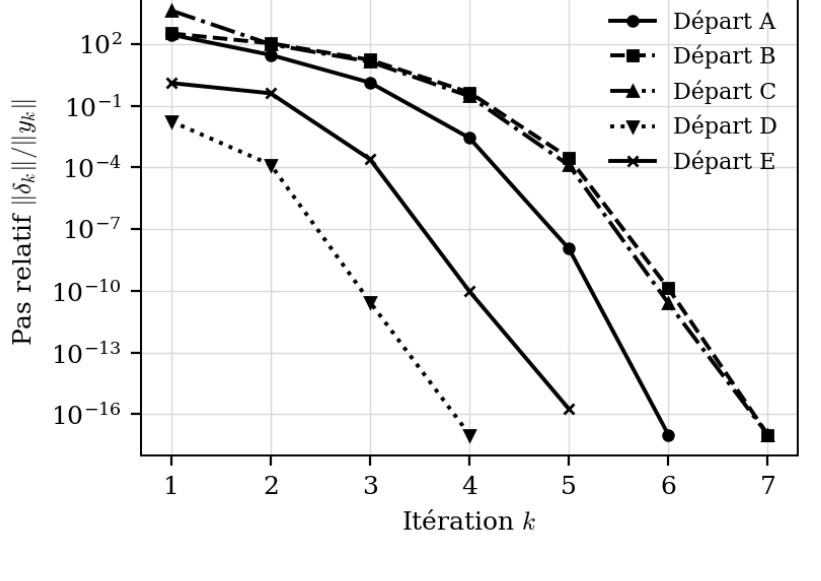
\includegraphics[width=\textwidth,height=4.5cm,keepaspectratio]{figures/fig5_newton.png}
        \end{column}
    \end{columns}
    \takeaway{convergence \textbf{quadratique} : le pas chute de plus en plus vite.}
\end{frame}

\begin{frame}{Raideur : pourquoi Euler explicite échoue}
    \small
    Rapport des valeurs propres $\approx23{,}5/0{,}0197\approx1200$ : système \textbf{raide}. Euler explicite est stable seulement si $h<\dfrac{2}{|\lambda_{\max}|}\approx0{,}085$ jour.
    \vspace{0.1cm}

    \figfull[4.3cm]{figures/fig6_raideur.png}
    \takeaway{à $h=0{,}1$ j, la méthode explicite diverge (a) ; l'implicite reste stable, même à $h=1$ j (b).}
\end{frame}

\begin{frame}{Schéma retenu : Euler implicite résolu par \texttt{DGESV}}
    \[
    \big[I-h\,J(y_k)\big]\,\Delta y_k=h\,f(y_k),\qquad y_{k+1}=y_k+\Delta y_k
    \]
    \begin{columns}[T,onlytextwidth]
        \begin{column}{0.46\textwidth}
            \begin{itemize}
                \item Un système $3\times3$ par pas, résolu par \texttt{DGESV}.
                \item Stable pour tout $h$ ; ordre $1$ ; jamais de valeur négative (on remet à $0$).
                \item Point fixe $=$ équilibre (écart $\approx10^{-5}$ à $t=600$ j).
            \end{itemize}
        \end{column}
        \begin{column}{0.5\textwidth}
            \small\centering
            Erreur à $t=10$ j (référence : \texttt{Radau})\\[3pt]
            \begin{tabular}{c c c}
                \toprule
                $h$ (jour) & Erreur & Ordre\\
                \midrule
                $0{,}05$ & $0{,}92$ & $1{,}5$\\
                $0{,}025$ & $0{,}39$ & $1{,}2$\\
                $0{,}0125$ & $0{,}18$ & $1{,}1$\\
                \bottomrule
            \end{tabular}
        \end{column}
    \end{columns}
    \takeaway{l'ordre observé tend vers 1, conformément à la théorie : le schéma est fiable.}
\end{frame}

% ==============================================================================
\section{Résultats médicaux}

\begin{frame}{Primo-infection : un pic viral foudroyant}
    \small
    Départ : sujet sain ($T=1000$) et une trace de virus.
    \vspace{0.1cm}

    \figfull[4.6cm]{figures/fig8_infection_primaire.png}
    \takeaway{pic de $\approx1{,}7\times10^{4}$ virions/$\mu$L vers le jour 15, CD4+ tombés à $\approx49$ ; puis retour oscillant vers l'état chronique.}
\end{frame}

\begin{frame}{Efficacité du traitement}
    \begin{columns}[T,onlytextwidth]
        \begin{column}{0.4\textwidth}
            \small
            \begin{tabular}{c c l}
                \toprule
                $\eta$ & $\Rzero$ & Effet\\
                \midrule
                $50\,\%$ & $2{,}0$ & le virus persiste\\
                $70\,\%$ & $1{,}2$ & répit, puis remontée\\
                $95\,\%$ & $0{,}2$ & éliminé\\
                \bottomrule
            \end{tabular}
        \end{column}
        \begin{column}{0.56\textwidth}
            \small\vspace{0.1cm}
            \begin{itemize}
                \item $\eta=95\,\%$ : indétectable en $\approx20$ jours.
                \item $\eta<75\,\%$ : le virus revient, même après avoir été indétectable.
            \end{itemize}
        \end{column}
    \end{columns}
    \vspace{0.1cm}
    \figfull[3.6cm]{figures/fig11_traitement.png}
    \takeaway{le seuil de 75\,\% calculé au chapitre analytique se confirme par simulation.}
\end{frame}

\begin{frame}{Danger de l'arrêt du traitement}
    \begin{columns}[T,onlytextwidth]
        \begin{column}{0.68\textwidth}
            \small
            Traitement à $95\,\%$ jusqu'au jour 100, puis arrêt : les CD4+ reconstitués ($T\approx724$) servent de cibles au virus résiduel.
        \end{column}
        \begin{column}{0.28\textwidth}
            \centering\kpi{$\times18$}{rebond vs. niveau chronique}
        \end{column}
    \end{columns}
    \vspace{0.1cm}
    \figfull[3.9cm]{figures/fig13_amplification.png}
    \takeaway{rebond de $\approx1{,}2\times10^{4}$ virions/$\mu$L : l'observance du traitement doit être continue.}
\end{frame}

\begin{frame}{Quels paramètres cibler ? Sensibilité de $\Rzero$}
    \small
    $\Rzero$ est un produit/quotient de paramètres : $\beta,\,p,\,s$ ont un indice $+1$ ; $d,\,\delta,\,c$ un indice $-1$ (+1\,\% sur le paramètre $\Rightarrow$ $\pm1$\,\% sur $\Rzero$).
    \vspace{0.1cm}

    \figfull[4.0cm]{figures/fig14_sensibilite.png}
    \takeaway{réduire l'infectivité $\beta$ ou la production virale $p$, ou accélérer la clairance $c$, réduit $\Rzero$ de façon proportionnelle.}
\end{frame}

% ==============================================================================
\section{Modèle de population}

\begin{frame}{Modèle $S, I_1, I_2$ et nombre de reproduction}
    \begin{columns}[T,onlytextwidth]
        \begin{column}{0.54\textwidth}
            \footnotesize
            \[
            \begin{cases}
            \dot S=\Lambda_aN-\beta S\dfrac{I_1+\varepsilon I_2}{N}-\mu_aS\\[4pt]
            \dot I_1=\beta S\dfrac{I_1+\varepsilon I_2}{N}-(\sigma+\mu_a)I_1\\[4pt]
            \dot I_2=\sigma I_1-(\mu_2+\mu_a)I_2
            \end{cases}
            \]
            \small Incidence \textbf{standardisée} (division par $N$) : le nombre de partenaires ne dépend pas de la taille de la population.
        \end{column}
        \begin{column}{0.42\textwidth}
            \centering
            \begin{tikzpicture}[
                c/.style={rectangle,draw=navy,fill=lightbg,minimum width=1.3cm,minimum height=0.8cm,align=center,font=\scriptsize\bfseries},
                r/.style={-{Stealth[length=2mm]},color=navy,thick}]
                \node[c] (S) {$S$\\\tiny sains}; \node[c,right=0.9cm of S] (I1) {$I_1$\\\tiny infectés}; \node[c,right=0.9cm of I1] (I2) {$I_2$\\\tiny SIDA};
                \draw[r] (S)--node[above,font=\tiny]{$\beta$}(I1); \draw[r] (I1)--node[above,font=\tiny]{$\sigma$}(I2);
            \end{tikzpicture}
        \end{column}
    \end{columns}
    \vspace{0.2cm}
    \[
    \Rzero^{\mathrm{pop}}=\frac{\beta}{\sigma+\Lambda_a}\Big(1+\frac{\varepsilon\sigma}{\mu_2+\Lambda_a}\Big)=1{,}8
    \qquad\beta_c\approx0{,}133\qquad\text{prévalence endémique}\approx68\,\%
    \]
    \takeaway{même méthode NGM qu'au niveau du patient ; $\Rzero^{\mathrm{pop}}>1$ : l'épidémie s'installe sans intervention.}
\end{frame}

\begin{frame}{Scénarios d'intervention (à partir de l'an 30)}
    \begin{columns}[T,onlytextwidth]
        \begin{column}{0.5\textwidth}
            \small
            \begin{tabular}{l c}
                \toprule
                \textbf{Scénario} & $\Rzero^{\mathrm{pop}}$\\
                \midrule
                Sans intervention & $1{,}80$\\
                Prévention ($\beta\times0{,}5$) & $0{,}90$\\
                Traitement seul ($\mu_2=0{,}1$) & $2{,}07$\\
                Prévention + traitement & $1{,}04$\\
                \bottomrule
            \end{tabular}
            \vspace{0.2cm}
            \begin{itemize}
                \item Le traitement seul prolonge la vie donc la contagiosité.
            \end{itemize}
        \end{column}
        \begin{column}{0.48\textwidth}
            \footnotesize\textbf{Prévalence à 300 ans}\\[4pt]
            \begin{tikzpicture}[x=0.052cm]
                \foreach \y/\v/\l [count=\i] in {0/67.8/Sans intervention, 1/0.07/Prévention, 2/64.0/Traitement seul, 3/4.6/Prévention + traitement} {
                    \node[anchor=east,font=\tiny,text=mid] at (-0.2,{-\y*0.72}) {\l};
                    \fill[navy!85] (0,{-\y*0.72-0.2}) rectangle (\v,{-\y*0.72+0.2});
                    \node[anchor=west,font=\scriptsize\bfseries,text=navy] at ({\v+1},{-\y*0.72}) {\v\,\%};
                }
                \draw[gold,line width=1.2pt] (0,0.35) -- (0,-2.5);
            \end{tikzpicture}
        \end{column}
    \end{columns}
    \takeaway{la \textbf{prévention} est le levier décisif ($\Rzero<1$) ; le traitement seul ne bloque pas la transmission.}
\end{frame}

% ==============================================================================
\section{Performance}

\begin{frame}{Benchmark : BLAS/LAPACK contre Python naïf}
    \begin{columns}[T,onlytextwidth]
        \begin{column}{0.7\textwidth}
            \footnotesize
            \begin{tabular}{c r r r r r r}
                \toprule
                & \multicolumn{3}{c}{\textbf{Produit matriciel}} & \multicolumn{3}{c}{\textbf{Résolution $Ax=b$}}\\
                \cmidrule(lr){2-4}\cmidrule(lr){5-7}
                $n$ & Naïf (ms) & \texttt{DGEMM} & Gain & Naïf (ms) & \texttt{DGESV} & Gain\\
                \midrule
                $50$ & $6{,}3$ & $0{,}009$ & $\times720$ & $2{,}6$ & $0{,}026$ & $\times100$\\
                $100$ & $45{,}8$ & $0{,}048$ & $\times950$ & $19{,}6$ & $0{,}094$ & $\times210$\\
                $200$ & $380{,}8$ & $0{,}39$ & $\times980$ & $142{,}5$ & $0{,}45$ & $\times310$\\
                \bottomrule
            \end{tabular}
            \vspace{0.1cm}

            \tiny Mesures : Xeon 2,8 GHz (2 cœurs), OpenBLAS 0.3.34, \texttt{benchmark\_blas.py}.
        \end{column}
        \begin{column}{0.26\textwidth}
            \centering\kpi{$\approx\times10^{3}$}{gain de \texttt{DGEMM}}
        \end{column}
    \end{columns}
    \takeaway{de l'ordre de mille fois plus rapide pour le produit matriciel, plusieurs centaines pour la résolution de système.}
\end{frame}

\begin{frame}{Passage à l'échelle}
    \small
    (a) temps d'exécution en $n^3$ ; (b) débit en GFLOPS de \texttt{DGEMM} et \texttt{DGESV}.
    \vspace{0.1cm}

    \figfull[4.3cm]{figures/fig19_benchmark_perf.png}
    \takeaway{\texttt{DGEMM} (niveau 3) garde un débit élevé et stable ; \texttt{DGESV} progresse avec $n$ à mesure que la part de niveau 3 grandit.}
\end{frame}

% ==============================================================================
\section*{Conclusion}

\begin{frame}{Conclusion : les chiffres clés}
    \vspace{0.2cm}
    \centering
    \begin{tabular}{c c c}
        \kpi{$\Rzero=4$}{sans traitement} & \kpi{$\eta_c=75\,\%$}{efficacité minimale} & \kpi{$\approx53$ j}{période des oscillations}\\[8pt]
        \kpi{$\times18$}{rebond après arrêt} & \kpi{$\Rzero^{\mathrm{pop}}=1{,}8$}{prévention décisive} & \kpi{$\times10^{3}$}{gain BLAS/LAPACK}\\
    \end{tabular}
    \vspace{0.3cm}

    \raggedright\small
    \begin{itemize}
        \item MKL, BLAS et LAPACK : une pile cohérente, appelée directement depuis Python.
        \item \texttt{DGEEQU}, \texttt{DGESV} et Euler implicite : calcul stable d'un système raide.
    \end{itemize}
    \takeaway{un modèle simple, des outils d'algèbre linéaire fiables, et des conclusions médicales claires.}
\end{frame}

\begin{frame}{Limites et perspectives}
    \begin{columns}[T,onlytextwidth]
        \begin{column}{0.5\textwidth}
            \textbf{\color{navy}Limites}
            \medskip
            \begin{itemize}
                \item Pas de réponse immunitaire adaptative, de cellules latentes ni de résistances.
                \item Population : mélange homogène ; $\beta$ calibré pour $\Rzero=1{,}8$ ; le traitement n'agit que sur $\mu_2$.
                \item Euler implicite d'ordre 1.
                \item Benchmark : un seul matériel ; OpenBLAS et MKL non comparés.
            \end{itemize}
        \end{column}
        \begin{column}{0.46\textwidth}
            \textbf{\color{navy}Perspectives}
            \medskip
            \begin{itemize}
                \item Intégrateur raide d'ordre supérieur (BDF, Radau).
                \item Comparer MKL et OpenBLAS selon le nombre de threads.
                \item Modèles spatiaux (EDP) avec solveurs LAPACK de bande.
                \item Exécution sur GPU (cuBLAS).
            \end{itemize}
        \end{column}
    \end{columns}
\end{frame}

\begin{frame}[plain]
    \begin{tikzpicture}[remember picture,overlay]
        \fill[navy] (current page.south west) rectangle (current page.north east);
        \node[text=white,font=\fontsize{34}{38}\selectfont\bfseries] at ($(current page.center)+(0,0.6cm)$) {Merci de votre attention};
        \draw[gold,line width=1.6pt] ($(current page.center)+(-2.2cm,-0.2cm)$) -- ($(current page.center)+(2.2cm,-0.2cm)$);
        \node[text=white!85,font=\Large] at ($(current page.center)+(0,-1.0cm)$) {Questions ?};
        \node[text=white!60,font=\scriptsize] at ($(current page.south)+(0,0.9cm)$) {Groupe 5 -- ENSGMM1 -- UNSTIM (Abomey)};
    \end{tikzpicture}
\end{frame}

\end{document}
